\documentclass[10.5pt,a4paper]{ctexart}
\usepackage{geometry}
\geometry{left=2.1cm,right=2.1cm,top=2.0cm,bottom=2.1cm}
\usepackage{amsmath,amssymb,amsfonts}
\usepackage{graphicx}
\usepackage{booktabs}
\usepackage{array}
\usepackage{xcolor}
\usepackage{hyperref}
\usepackage{enumitem}

\setlist{nosep,leftmargin=1.5em}
\setlength{\parskip}{4pt}

\hypersetup{
    colorlinks=true,
    linkcolor=blue!60!black,
    urlcolor=blue!60!black,
    pdftitle={Conditional Value Memory Research Proposal v5},
    pdfauthor={Project Collaborators}
}

\title{\textbf{面向高效语言模型的条件价值查表记忆：\\
交叉临界律、现象学理论与跨层多粒度容量分配}\\[6pt]
\large —— 从研究背景、机制诊断到全词表 Bridge 与 125M 规模化实验的完整研究方案（v5 详细协作版）}
\author{项目代码与数据仓库：\texttt{Rinck1/value-memory-crossover}（\texttt{docs/ICML\_Research\_Proposal\_v5.pdf}）}
\date{版本日期：2026-11-23}

\begin{document}
\maketitle

\begin{abstract}
\noindent
本文档是一份\textbf{自包含（self-contained）的完整研究方案与实验汇总报告}，旨在让新加入的合作者无需回溯历史讨论即可全面掌握本课题的\textbf{动机背景、理论边界、诊断排雷、构造性方法（MP-VE 与 \texttt{U123}）、全套本地与全词表实测结果，以及下一阶段 \texttt{125M × 2.5B} 云端实验计划}。核心结论如下：
\begin{enumerate}
    \item \textbf{精确问题定位：} 在注意力价值流（Value Stream）及残差流中引入离散 N-gram 查找表，可在\textbf{等激活计算量与推理延迟受限（Equal Active FLOPs）}前提下显著降低语言模型困惑度（Perplexity / NLL）；但在\textbf{等总参数量（Equal Total Weights）}条件下，中短训练尺度下加宽密集主干仍更占优。
    \item \textbf{交叉机制与排雷诊断：} 单字表（1-gram）在 $<100$ 次训练观测的稀疏位置领先，双字表（2-gram）在 $100\text{--}999$ 次观测后反超；此前小词表 \texttt{1000+} 桶表面混杂由 \texttt{<UNK>} 词对（占 $51.9\%$ 类型 / $68\text{--}72\%$ 位置）引起，剔除 \texttt{<UNK>} 后一致翻转为双字表胜出。同时证实独立双字表直接加门控失效、逐行稀疏 \texttt{SparseRowAdam} 在本设定显著劣于 Dense Adam。
    \item \textbf{三个可检验现象学模型：} 建立并校准 KKT 显存约束三档分配（\texttt{0/r/d}）、Zipf--Heaps 训练交叉时间 $T_{\text{cross}}$ 三项分解，以及跨层共享 \texttt{U1} 梯度方差缩减假设。
    \item \textbf{方法与跨尺度实测：} 最终构造的 \texttt{U123} 架构（跨层共享宽表 + 双路注入 + \texttt{2g/3g} 精确高敏银行 + pre-head 读出 + 10\% 前缀计数路由）在 $L=4,w=32,V=6{,}000$（3 seeds）以少 $35\%$ 表参击败严格匹配控制臂 \texttt{CTRL\_hs}（$5.3190\pm0.0068$ vs $5.3349\pm0.0022, \, t=+4.96$）；推至真实 GPT-2 词表 $V=50{,}257$ 的 $30\text{M}$-token Bridge 中，\texttt{U123} 达到 \textbf{4.8234}（对比 \texttt{plain\_d256} $4.9855$ 降低 \textbf{0.1621 nats}），并在 $30\text{M}$ tokens 节点完成对未剪枝哈希对照 \texttt{CTRL\_hs}（$4.8324$）的交叉反超。
\end{enumerate}
\end{abstract}

\tableofcontents
\newpage

% ============================================================
\section{研究背景、文献争议与本文精确切入点}
% ============================================================

\subsection{为什么需要在 Transformer 中引入“条件价值查表记忆”？}
标准自回归语言模型的知识存储与推理计算高度耦合在 Transformer 的前馈网络（FFN）与注意力投影矩阵（$W_Q, W_K, W_V, W_O$）中：要想扩大静态模式与搭配记忆容量，就必须加宽隐藏层 $d$ 或加深层数 $L$，从而按 $\mathcal{O}(L d^2)$ 成倍增加每 token 的激活 FLOPs 与自回归推理延迟。近年来，一条备受关注的解耦路线是\textbf{条件价值查表记忆（Lookup-Based Value / Residual Memory）}：直接根据当前词元 $w_t$ 或局部 N-gram $(w_{t-1}, w_t)$，以 $\mathcal{O}(1)$ 内存查表方式检索一个轻量级高维向量银行 $E[\text{key}]$，并将其注入注意力价值向量 $V^{(\ell)} = W_V^{(\ell)} h^{(\ell)} + \Delta V_{\text{mem}}^{(\ell)}$（或残差流）。代表性工作包括：
\begin{itemize}
    \item \textbf{按单字索引（1-gram）路线：} Speedrun 价值嵌入、\textbf{Bank of Values}（He et al., 2026，验证末三分之一深层放置可在 135M/780M 上省参并获益）、\textbf{X-GRAM}（Chen et al., 2026，指出 2M 表中仅 $7.3\%$ 表项收到 $>100$ 次更新，提出高频词建独立表、其余压缩）、\textbf{MoVE}（Li, 2026）与 \textbf{Memory Attention}（Kang, 2026）。
    \item \textbf{按局部序列索引（2-gram / N-gram）路线：} \textbf{DeepSeek Engram}（Cheng et al., 2026，使用带 RMSNorm 点积上下文门控的哈希 N-gram 查表注入）、modded-nanogpt bigram-hash、\textbf{Scone}（Yu et al., 2025）、\textbf{LongCat}（Liu et al., 2026，将 N-gram 表扩展至 $>30\text{B}$ 参数并在 $300\text{B}$ tokens 后反超每层单字表）以及 \textbf{Over-Tokenized Transformers}（Huang et al., 2025，报告短中程下纯 2-gram 表劣于 1-gram 表）。
\end{itemize}

\subsection{现有文献的明显分歧与“尚未回答的空白”}
不同论文对“1-gram 表好还是 2-gram 表好”给出了截然相反的经验结论：Over-Tokenized Transformers 与 Hash Layers（Roller et al., 2021）报告 1-gram 胜出；MoME（Li et al., 2026）在 135M 规模上报告单字 Value Embedding 与 Bigram 查表\textbf{打成平手}；而 LongCat 在 $300\text{B}$ tokens 极长训练后却报告 N-gram 表\textbf{明显领先}。造成表面矛盾的根本原因在于文献普遍缺乏统一的微观机制变量：
\begin{enumerate}
    \item 缺少\textbf{按词对累计训练次数（sightings $c$）与文本覆盖份额拆分}的定量比较；
    \item 缺少关于\textbf{哈希碰撞（表行数 $M$）、模型宽度 $d$、总训练量 $T$} 何时允许或阻断交叉的相图检验；
    \item 在架构工程上，缺乏同时解决\textbf{“低频行梯度噪声污染”}、\textbf{“长尾碰撞误差”}、\textbf{“大规模全词表显存爆炸（若为 $V=50{,}257$ 建 11.5M 全双字表需 $8.8\text{B}$ 参数）”}，且能用\textbf{严格控制变量（matched-adapter control）}证实增益来源的设计。
\end{enumerate}

\subsection{本项目的核心定位：严格划分两类对比预算}
为了避免将“靠堆砌总参数换取的收益”混淆为架构优势，本项目从立项第一天起就强制区隔两种对比锚点（任何论文与实验汇报均须独立展示这两条基线）：
\begin{itemize}
    \item \textbf{Equal Active FLOPs（主锚点）：} 在相同的骨干宽度 $d$、深度 $L$ 与近乎相等的每 token 激活计算量下（如 $d=256$ 主干 + 查表 vs 纯 $d=256$ 主干），验证查表记忆如何利用廉价 $\mathcal{O}(1)$ 内存读取换取显著更低的困惑度。这是边缘端与大吞吐解码部署的真实场景。
    \item \textbf{Equal Total Weights（对照边界）：} 当把查表参数折算进总参数并允许主干自由加宽至同等总参数（例如 $L=4, w=32$ 对比加宽主干 $w=88$，或 $V=50{,}257$ 处 $d=256$ 对比 $d=384$）时，在 $6\times$ / $2.25\times$ 更高的激活算力代价下，加宽密集主干仍显著领先查表方案。我们\textbf{诚实汇报该边界，不主张 Equal-Weights 无条件胜出}。
\end{itemize}

% ============================================================
\section{微观机制实证与关键排雷诊断}
% ============================================================

\subsection{Sighting-Count 交叉律与 \texttt{<UNK>} 输入混杂的澄清}
在对齐 FineWeb 验证集每个位置的上下文词对 $(w_{t-1}, w_t)$ 在训练中累计被更新的次数 $c$ 后，我们在三个词表尺度 $V \in \{1{,}500, 3{,}000, 6{,}000\}$（3 seeds，300 步）上测得一致的分桶规律（图~\ref{fig:fig1}）：
\begin{itemize}
    \item \textbf{低频区（\texttt{pc\_0}，\texttt{pc\_1}，\texttt{pc\_10}，$c < 100$）：} 双字表由于单行梯度更新稀疏、方差大，稳定落后于共享同一词元统计的 1-gram 单词表（例如 $V=6{,}000$ 上 \texttt{engram - word} 在 \texttt{pc\_0/1/10} 分别为 $+0.0490, +0.0484, +0.0230$ nats）。
    \item \textbf{成熟交叉带（\texttt{pc\_100}，$100 \le c < 1000$）：} 词对向量完成收敛并脱离噪声区，2-gram 开始反超 1-gram（$V=3{,}000$ 上 $-0.0248$ nats，$V=6{,}000$ 上 $-0.0143$ nats）。
    \item \textbf{解开 \texttt{pc\_1000} 桶的表面矛盾（\texttt{unk\_filtered\_eval.json}）：} 在早期包含全部评估位置的统计中，$V=1{,}500/3{,}000/6{,}000$ 的 \texttt{1000+} 桶出现反常混杂（\texttt{engram - word} 为 $+0.0142 / -0.0024 / +0.0172$）。定量审计发现：\textbf{在截断词表下，$51.94\%$（$67/129$）的训练高频词对类型与 $67.83\%\text{--}71.52\%$ 的验证集位置本身包含 \texttt{<UNK>} 伪词元}（仅 $(\texttt{<UNK>}, \texttt{<UNK>})$ 一对就出现 $69{,}954$ 次，完全丧失细粒度语法上下文）。当仅在\textbf{非 \texttt{<UNK>} 真实词对}上评估时，\texttt{pc\_1000} 的 \texttt{engram - word} 一致翻转为清晰的 Pair 胜出：$-0.0380$（$V=1{,}500$）、$-0.0501$（$V=3{,}000$）、$-0.0241$（$V=6{,}000$）nats；而 \texttt{MP-VE - word} 优势则进一步扩大至 $-0.0506 / -0.0580 / -0.0456$ nats。因此，我们谨慎将交叉界定为\textbf{约 100 次更新左右的过渡区间}而非刻板阈值。
\end{itemize}

\begin{figure}[htbp]
    \centering
    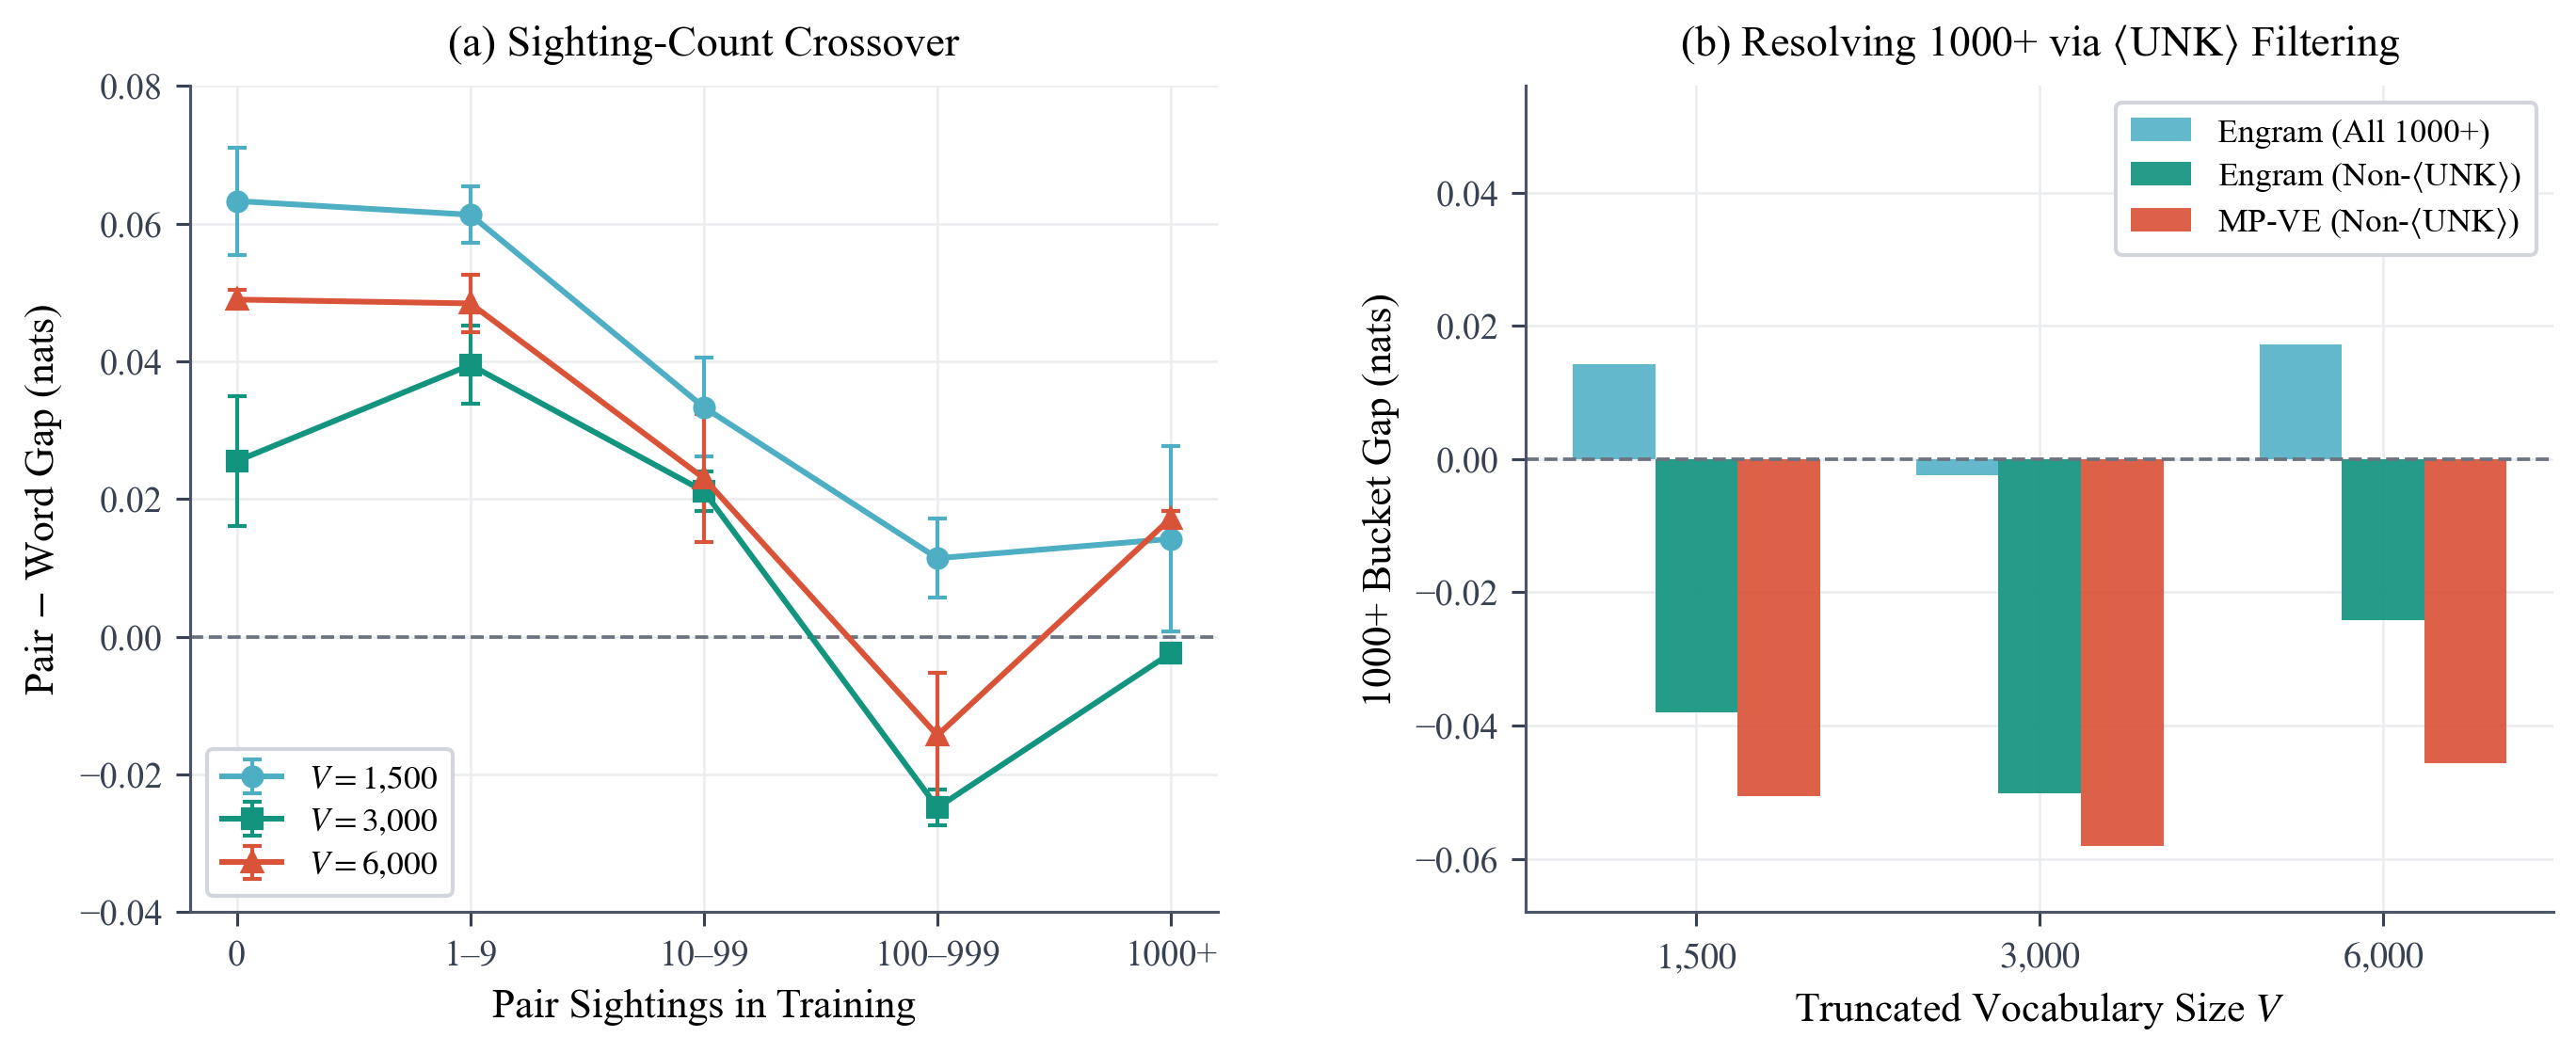
\includegraphics[width=0.92\linewidth]{../figs_v5/fig1_crossover.png}
    \caption{Fig.~1：Word vs Pair 按训练频次分桶的性能差值（$V \in \{1{,}500, 3{,}000, 6{,}000\}$，3 seeds $\pm$ s.e.m.，负值代表 Pair 更优）。$<100$ 次桶由 1-gram 领先，\texttt{100--999} 桶由 2-gram 反超；剔除小词表特有的 \texttt{<UNK>} 词对混杂后，\texttt{1000+} 桶同样呈现清晰的 2-gram 优势。}
    \label{fig:fig1}
\end{figure}

\subsection{排雷诊断一：上下文门控失灵与单表成熟度门控负结果}
早期设计容易假设“用输入相关的上下文门控（如 Engram 的 RMSNorm 点积门控）就能自动关闭噪声行，或在独立 2-gram 表上直接挂接成熟度门控”。我们在 Block~A 与 Block~F（3 seeds，\texttt{local\_suite\_results.json}）中对其进行了证伪检验（图~\ref{fig:fig6}(a)）：
\begin{enumerate}
    \item \textbf{Engram Full 上下文门控实测与频次无稳定相关（Block~F）：} 完整版 Engram（带 RMSNorm 点积门控）与词对训练频次的 Pearson 相关系数在 150 步为 $r=-0.034\pm0.131$、300 步为 $r=-0.046\pm0.123$，5 个频次桶的门控均值几乎完全平坦地停留在 $0.410\text{--}0.440$（RMSNorm 归一化抹平了低频欠训练向量与高频成熟向量的范数差异）；仅有去掉归一化的 \texttt{core} 变体保住了弱正相关（$r=+0.326\pm0.101$，但 \texttt{pc\_0} 开度仍偏高达 $0.535$）。
    \item \textbf{零先验均匀初始化证明优化器本能（Block~E）：} 当改用直接按频次桶参数化且权重全零初始化（初始 sigmoid 全部 $=0.500$）的 5 桶直通门控时，反向传播在 $V=1{,}500/3{,}000/6{,}000$ 上均自发将 \texttt{1--9} 欠训练桶压低至 $0.12\text{--}0.16$，将 \texttt{100+} 成熟桶拉升至 $0.89\text{--}1.00$。
    \item \textbf{没有 1-gram 兜底的单表成熟度门控失效（Block~A，负结果）：} 直接对单挂的 \texttt{engram\_full}（$5.5405\pm0.0068$）施加乘法或加法成熟度门控均导致性能持平或显著恶化：\texttt{engram\_mat\_mul} $=5.5760\pm0.0067$，\texttt{engram\_mat\_add} $=5.6034\pm0.0024$，\texttt{engram\_b5\_mul} $=5.5403\pm0.0016$。原因在于关掉低频 2-gram 后位置失去基础表达，且低频行更难翻身形成\textbf{梯度自锁}。仅当将其重构为\textbf{双粒度互补（Word 1-gram 兜底 + Pair 2-gram 按成熟度路由）}时，损失才大幅降至 $5.4928\pm0.0102$。
\end{enumerate}

\begin{figure}[htbp]
    \centering
    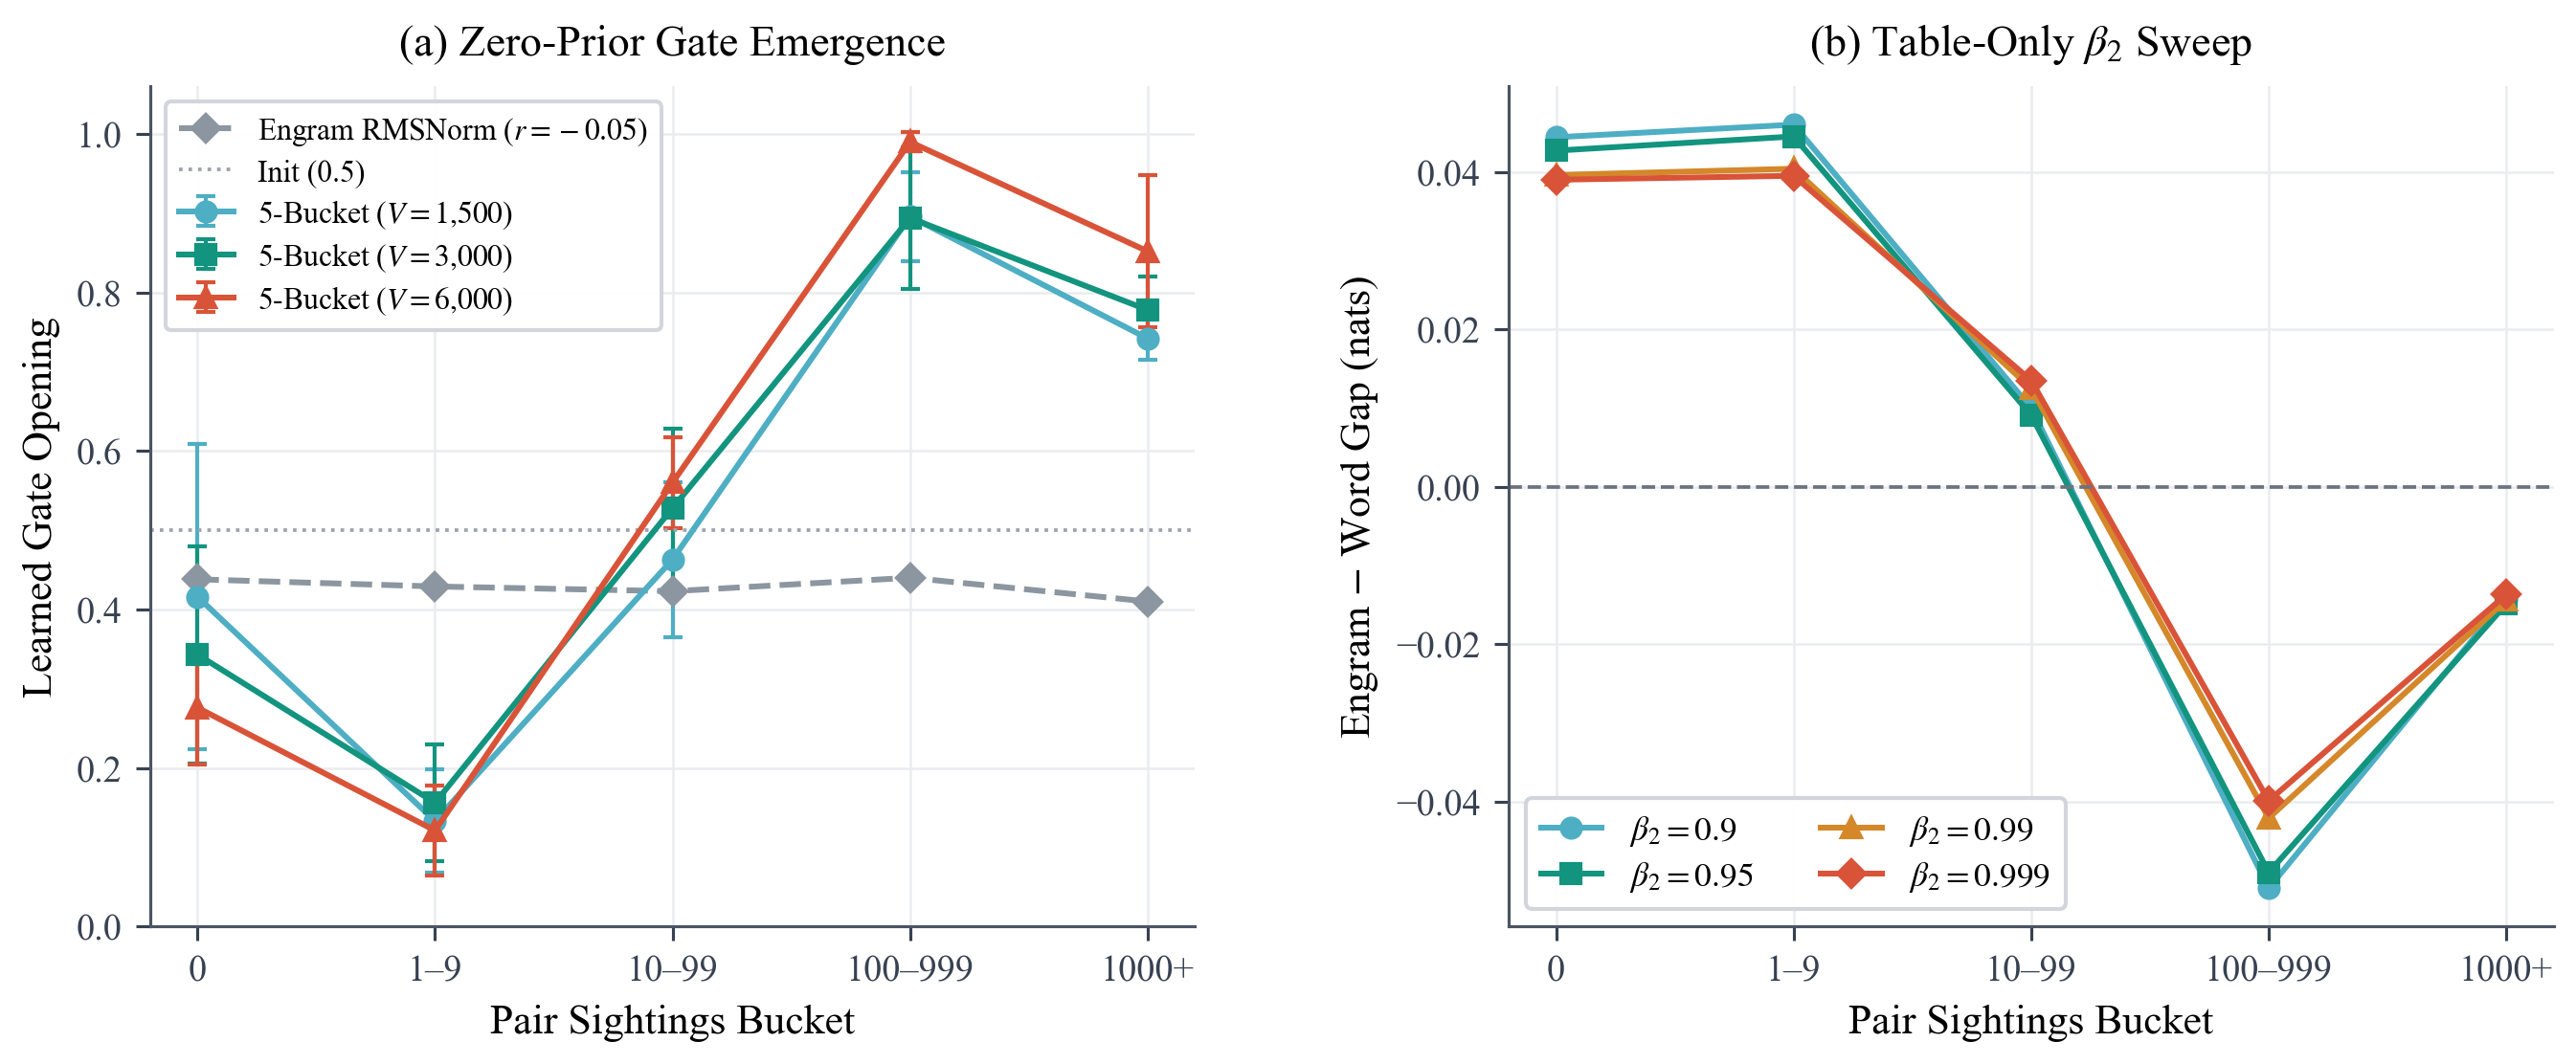
\includegraphics[width=0.92\linewidth]{../figs_v5/fig6_gates_beta2.png}
    \caption{Fig.~6：(a) 全 0.5 均匀初始化的 5 桶门控自发收敛分化，对比平坦失效的 Engram Full 点积门控；(b) 查表专属 $\beta_2$ 在 $[0.9, 0.999]$ 跨越 $100\times$ 后交叉带位置稳定，证伪 $c^\star \propto (1-\beta_2)^{-1}$ 猜测。}
    \label{fig:fig6}
\end{figure}

\subsection{排雷诊断二：稀疏优化器（\texttt{SparseRowAdam}）为何显著输给 Dense Adam？}
在常规工程直觉中，查表参数极大且每次 batch 仅访问少部分行，理应采用只对命中行更新且按行独立累计步数 $t_{\text{row}}$ 的稀疏 Adam（\texttt{SparseRowAdam}）以节省算力并保持统计无偏。我们在检查并修复早期代码中的 \texttt{index\_add\_} 梯度汇聚缺陷后（\texttt{p0\_results.json}，3 seeds，$L=4,w=32,V=6{,}000$），对 Dense Adam 与四种 \texttt{SparseRowAdam} 变体进行了配对实验：
\begin{itemize}
    \item \texttt{mp\_ve\_last2\_dense}（Dense Adam 主线）：3-seed 前 3 种子同配对下均值为 \textbf{5.3442 $\pm$ 0.0089}（5-seed 为 $5.3440\pm0.0070$）；
    \item \texttt{sparse\_row\_t\_fixed}（修复后的精确逐行计步）：\textbf{5.3626 $\pm$ 0.0111}，配对差达 \textbf{$-0.0184 \pm 0.0023$ nats ($t = -13.60$)}；
    \item \texttt{sparse\_global\_t} ($5.3627$)、\texttt{sparse\_decay\_m\_only} ($5.3721$)、\texttt{sparse\_decay\_v\_only} ($5.3569$) 均稳定落后 Dense Adam。
\end{itemize}
\textbf{机理归因：} 当某个稀有词对仅被命中 $t_{\text{row}}=1\text{--}3$ 次时，精确逐行偏差修正 $\frac{1}{1-\beta_1^{t_{\text{row}}}}$ 与 $\frac{1}{\sqrt{1-\beta_2^{t_{\text{row}}}}}$ 会对其高度噪杂的早期梯度施加接近满幅的大步长，引发低频表行震荡；反之，Dense Adam 对未命中行自动施加动量自然衰减 $m \leftarrow \beta_1 m$ 并使用全局平滑时间步 $t_{\text{global}}$，对偶发梯度噪声起到了强正则化作用。据此，我们在所有桥接实验与 125M 脚本中\textbf{显式规定表参数采用 Dense AdamW 策略并诚实计算其优化器开销}。

% ============================================================
\section{三个可检验的现象学理论模型（Section 2 核心理论框架）}
% ============================================================

为了避免“零自由参数严谨推导”在审稿中遭到挑剔，我们将论文理论架构定位为\textbf{三个“现象学模型 + 定量预测 + 判别实验（Model + Prediction + Test）”}，逐一给出各自成立与退化的条件区间。

\subsection{现象学模型 1：KKT 显存约束下的三档容量分配（\texttt{0 / r / d}）}
设词对 $(w_{t-1}, w_t)$ 在总训练过程中获得 $c$ 次有效更新，其被分配的有效表示维度为 $r_c \in [0, d]$。对不同频次词对在显存与参数总量约束 $\sum_{u} r_u \le M_{\text{tab}}$ 下极小化总期望超额风险（包含低秩近似偏差 $\varphi(r_c/d)$、有限样本随机梯度方差 $B c^{-\nu} (r_c/d)^\gamma$ 与长尾行平均显存占用成本 $\mu T / c \cdot r_c$）：
\begin{equation}
\min_{\{r_c \in [0, d]\}} \sum_c N(c)\left[\sigma_{\text{bias}}^2\cdot \varphi\!\left(\frac{r_c}{d}\right) + B\, c^{-\nu} \left(\frac{r_c}{d}\right)^\gamma + \mu \frac{T}{c} \cdot r_c\right]
\end{equation}
\begin{itemize}
    \item \textbf{规范性解释（Rationalization）：} KKT 互补松弛条件自然诱导三个运行区间——当 $c < c_{\text{lo}}$ 时最优解触及下界 $r_c^\star = 0$（完全剪枝退回共享 1-gram 单词表，避免引入纯噪声）；当 $c_{\text{lo}} \le c < c_{\text{hi}}$ 时存在中间平滑过渡区，工程上离散化为低秩投影 $r = d/4$；当 $c \ge c_{\text{hi}}$ 时触及上界 $r_c^\star = d$（全秩独立表示）。
    \item \textbf{带宽比的条件性范围：} 中频带跨越宽度 $c_{\text{hi}}/c_{\text{lo}}$ 并不是无条件常数 $10\times$，而取决于主导成本项——当\textbf{随机方差项 $B c^{-\nu}$ 主导}时，$c_{\text{hi}}/c_{\text{lo}} \approx (\varphi'(0^+)/\varphi'(1))^{1/\nu} \approx 3.5^2 \approx \mathbf{10\text{--}12\times}$；当\textbf{显存租金项 $\mu T/c$ 主导}时，该比值退化至 $\approx \varphi'(0^+)/\varphi'(1) \approx \mathbf{3\text{--}5\times}$。这一理论边界正好与实测经验区间 $[10, 100)$ 相自洽。
\end{itemize}

\paragraph{相图、宽度弱可辨识性与 $\beta_2$ 检验（Block B, Block C, \texttt{theory\_cstar\_analysis.json}）：}
\begin{enumerate}
    \item \textbf{$(M, T)$ 碰撞--方差相图（图~\ref{fig:fig23}(a)）：} 当哈希表行数 $M \le 2{,}048$ 时，碰撞误差 $\sigma_{\text{coll}}^2(V, M) \ge \sigma_{\text{ctx}}^2$，即使训练至 600 步（4.92M tokens）2-gram 仍持续落后 1-gram $+0.0162 \sim +0.0364$ nats（永不交叉）；唯有当 $M = 16{,}384$ 且训练达 $300\text{--}600$ 步时，相边界翻转并反超 $-0.0189$ nats。
    \item \textbf{宽度标度 $c^\star(d)$ 的弱可辨识区间与持出检验（图~\ref{fig:fig23}(b)）：} 随着主干宽度 $d$ 从 $16$ 增至 $128$，2-gram 在成熟桶 \texttt{pc\_100} 相对 Word 的净优势从 $-0.0490$ 单调收缩至 $-0.0157$（说明更宽模型中基础主干与 1-gram 能力变强，而更宽查表行所需校准更新量增大）；同时 \texttt{MP-VE} 相对 Word 的全局净增益在最宽处 $d=128$ 达到 $+0.0179$ nats（$5.4469$ vs $5.4648$）。然而通过严格区间辨识审计，在 \texttt{strict\_identified} 标准下所有宽度均未锁定唯一闭式斜率，$d\in\{16, 32, 64\}$ 属于\textbf{弱可辨识次线性区间}（$\alpha \approx 0.32$），而 $d=128$ 因两端噪声退化为不可辨识。在预注册持出宽度 $d=24, 48$ 上：\texttt{b\_500\_1000} 均保持正收益（$+0.01748$ 与 $+0.03459$ nats），\textbf{明确拒绝朴素线性假设 $\alpha=1.0$}（该假设预言 $d=48$ 处 $c^\star=1224.6$ 故 \texttt{b\_500\_1000} 必为负），但 $d=48$ 总体提前交叉于 $80$（提示宽模型下 1-gram 残差方差系数 $B$ 亦随之变化）。
    \item \textbf{证伪 $c^\star \propto (1-\beta_2)^{-1}$（图~\ref{fig:fig6}(b)）：} 保持主干 $\beta_2=0.95$ 不变、仅将查表 AdamW 的 $\beta_2$ 在 $[0.9, 0.999]$ 横跨 $100\times$ 变动后，交叉位置定性稳定落在 \texttt{pc\_10} 与 \texttt{pc\_100} 之间（仅幅值衰减约 $20\%$），证伪该时间常数假说。
\end{enumerate}

\begin{figure}[htbp]
    \centering
    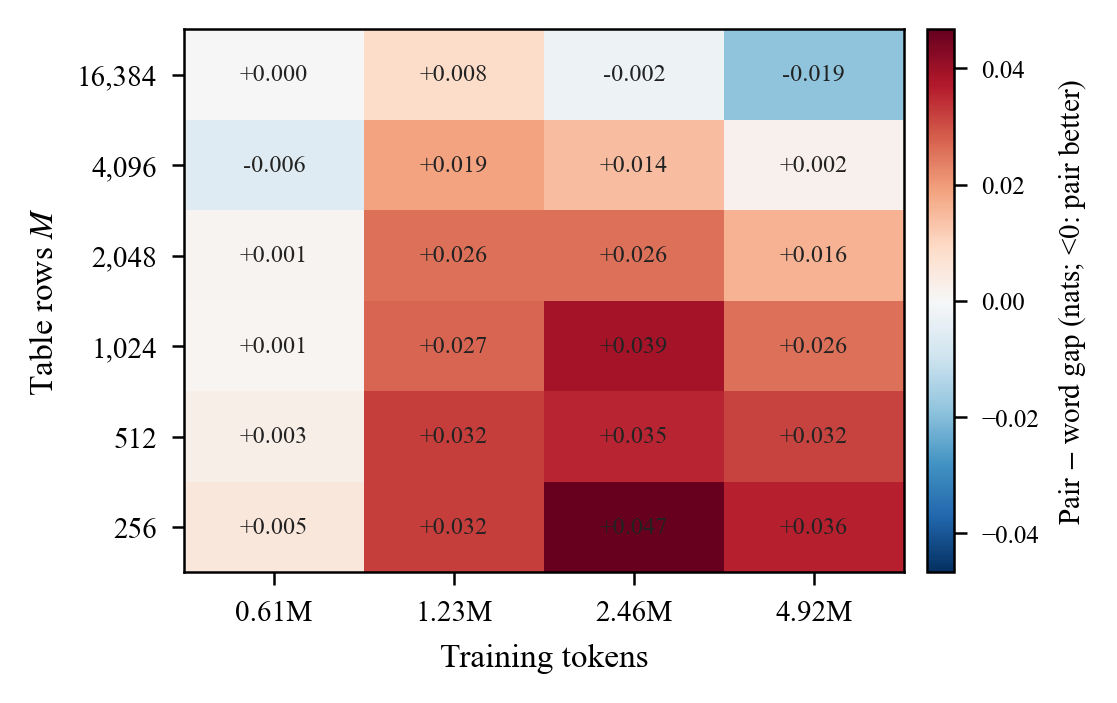
\includegraphics[width=0.49\linewidth]{../figs_v5/fig2_phase.png}\hfill
    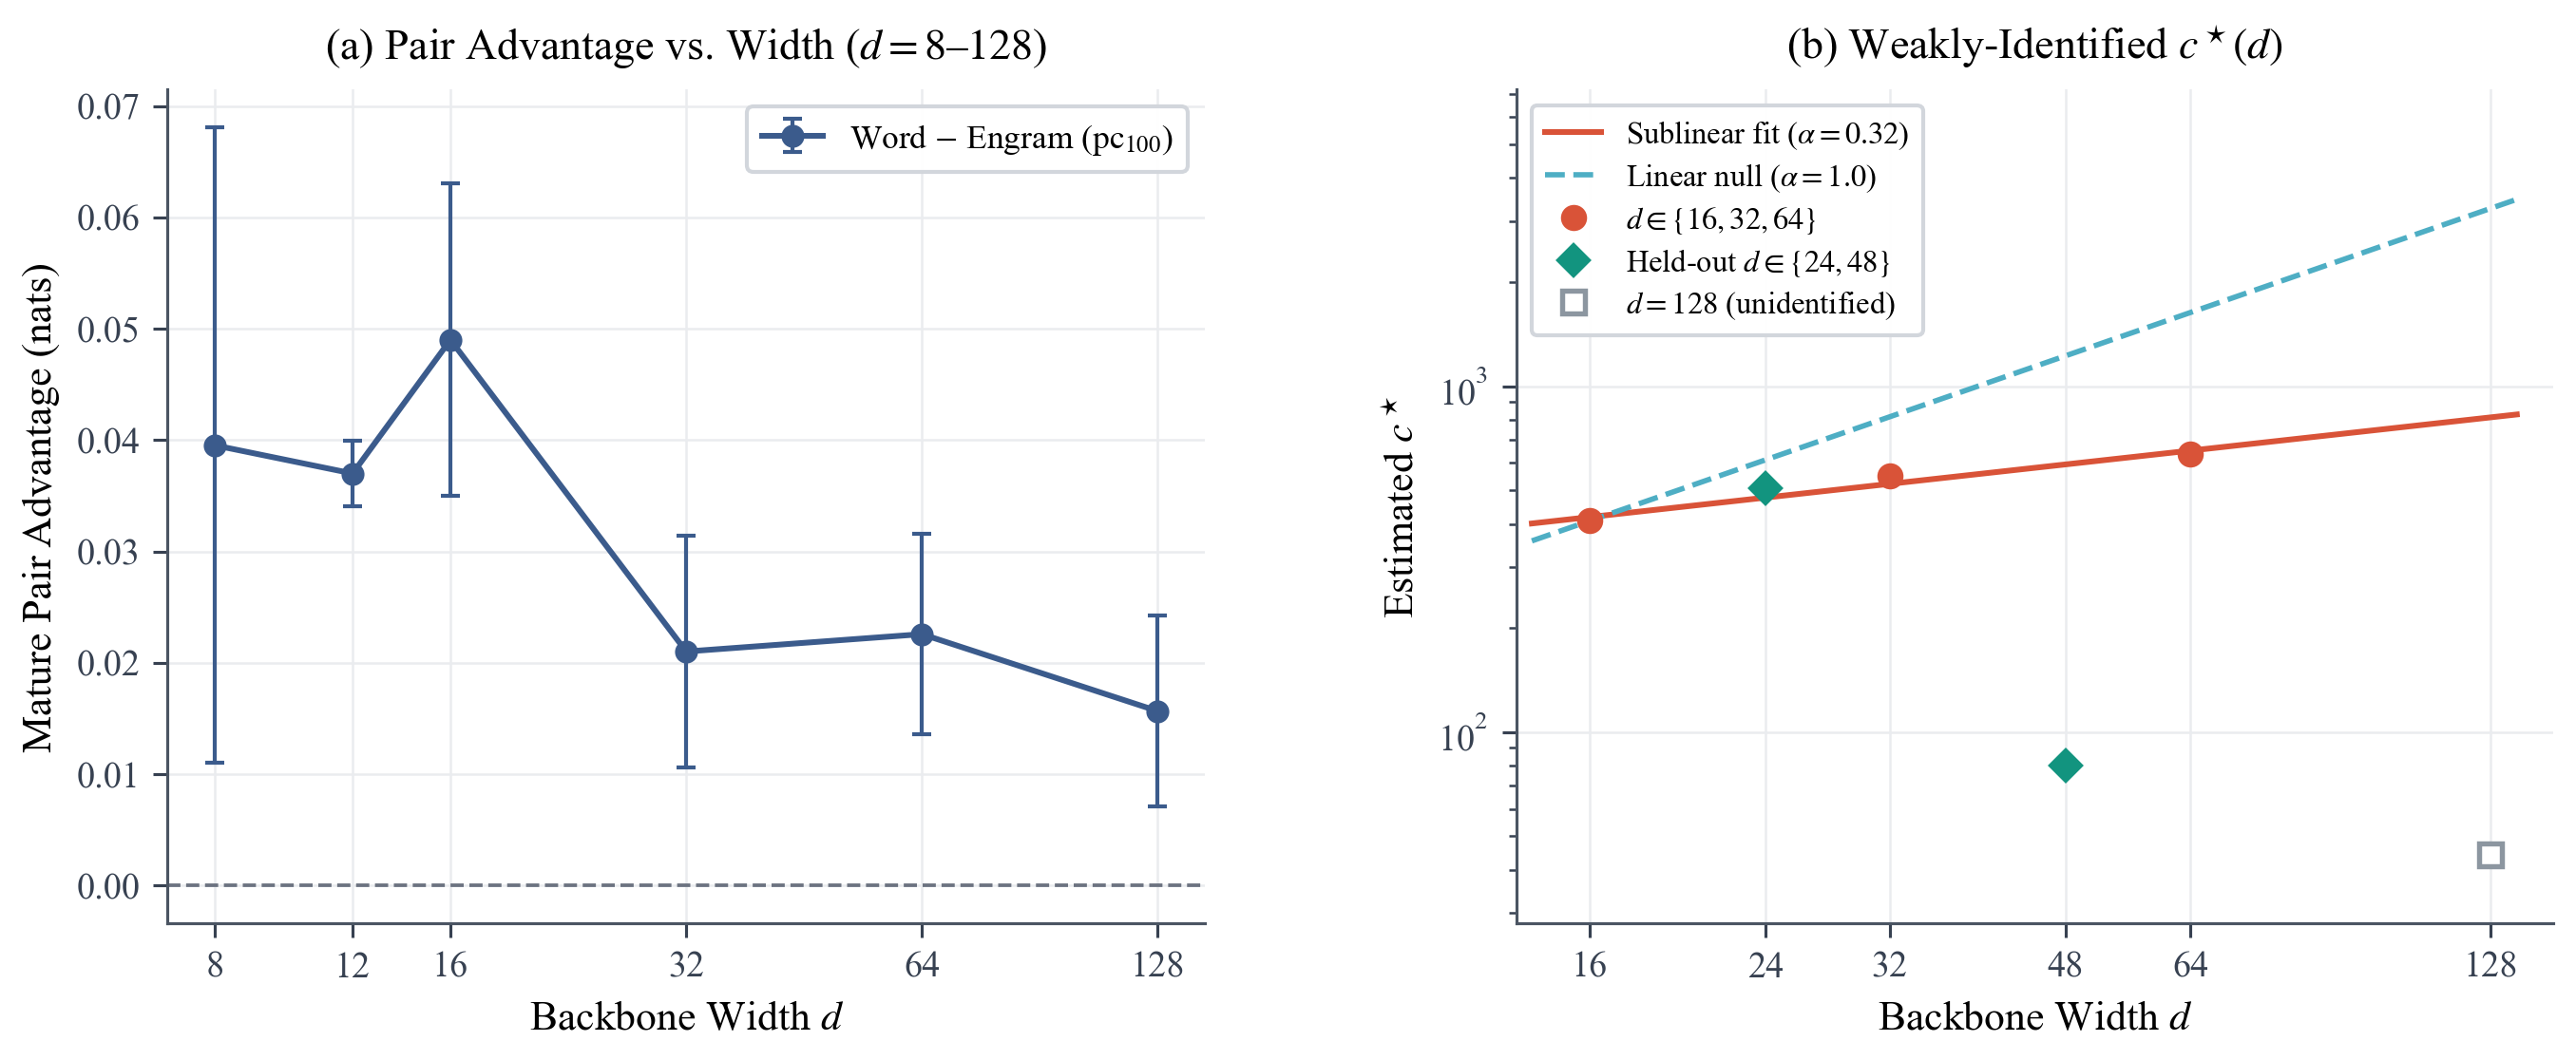
\includegraphics[width=0.49\linewidth]{../figs_v5/fig3_width_cstar.png}
    \caption{左（Fig.~2）：$V=1{,}500$ 上的 $(M, T)$ 碰撞--方差相图，仅当表行数 $M$ 与训练步数 $T$ 同时跨过阈值后 2-gram 才翻转胜出；右（Fig.~3）：高宽模型中 2-gram 单桶优势收缩，$c^\star(d)$ 在 $d=16\text{--}64$ 呈弱可辨识次线性增长（$\alpha\approx 0.32$），$d=24,48$ 持出检验拒绝线性 $\alpha=1.0$。}
    \label{fig:fig23}
\end{figure}

\subsection{现象学模型 2：Zipf--Heaps 训练交叉时间 $T_{\text{cross}}$ 三项分解}
在扩大至真实词表（$V=50{,}257$）并与高质量未剪枝基线比较时，多粒度精确表呈现典型的\textbf{“先输后赢”}轨迹（第 5 节 30M Bridge 中 \texttt{U123 - CTRL\_hs} 从 7.5M 时的 $-0.0183$ 一路追平并在 30M 交叉翻正为 $+0.0090$）。我们将总训练步 $T$ 上的这一差距分解为三项竞争效应：
\begin{equation}
\Delta \mathcal{L}_{\text{U123 vs CTRL\_hs}}(T) \;=\; \underbrace{+\Delta_{\text{prune}}(T)}_{\text{剪枝去除 }\texttt{pc\_0}\text{ 噪声}} \;+\; \underbrace{\Delta_{\text{exact}}(U(T), M)}_{\text{精确双三元组消除哈希碰撞}} \;-\; \underbrace{\Delta_{\text{warmup}}(r, T)}_{\text{宽银行与低秩投影初期预热税}}
\end{equation}
这一分解无需凭空猜测函数细节，可通过我们在代码库已实现的三重控制臂阶梯实测拆解：
\[\texttt{CTRL\_word} \;\xrightarrow{+\,\text{适配头与哈希 }2g/3g}\; \texttt{CTRL\_hs} \;\xrightarrow{+\,\text{成熟度剪枝}}\; \texttt{CTRL\_hs\_pruned} \;\xrightarrow{+\,\text{精确银行防碰撞}}\; \texttt{U123}\]
其中 \texttt{CTRL\_hs\_pruned - CTRL\_hs} 精确度量第一项“去污染”，而 \texttt{U123 - CTRL\_hs\_pruned} 则精确剥离第二项“精确防碰撞”减去第三项“预热税”后的净收益。

\subsection{现象学模型 3：跨层共享表（\texttt{U1}）梯度方差缩减假设}
在架构升级消融中我们观测到一个关键现象：\textbf{跨全层共享一张更宽的公共记忆表（\texttt{U1}）贡献了相对原始 \texttt{MP-VE} 增益的主力；而诸如 3-gram 或 pre-head readout（\texttt{U3}）等改进单独加入未共享架构时作用温和，一旦并入跨层共享框架后效果叠加放大}。现象学机制解释如下：当同一词对行跨 $L$ 层复用并由每层独立轻投影 $W^{(\ell)}$ 接入时，同一词频 $c$ 在单次前向中聚集了来自 $L$ 个深度的反向梯度；若共享语义信号方向相干、而各层残留梯度噪声的跨层相关系数为 $\rho_{\text{noise}} \in [0, 1)$，则单步有效信噪比由孤立分层表的 $1$ 提升为：
\begin{equation}
\text{SNR}_{\text{eff}}(L) \;\propto\; \frac{L}{1 + (L - 1)\rho_{\text{noise}}}
\end{equation}
\textbf{可证伪检验：} 该假设预测跨层共享对低频/中频长尾表的收敛增益应随有效层数 $L \in \{2, 4, 6\}$ 呈次线性递增且可在梯度余弦测量中观测到非饱和噪声相关性；该项检验脚本已在 \texttt{experiments/run\_theory\_tests\_L\_M\_rho.py} 就绪，将在下一阶段与云端实验并线补齐。

% ============================================================
\section{方法架构演进与严格多 Seed 归因验证}
% ============================================================

\subsection{从 \texorpdfstring{\texttt{MP-VE}}{MP-VE} 到 \texorpdfstring{\texttt{U123}}{U123} 的四步演进}
对于初次接触本代码库的合作者，可以将本项目的核心方法矩阵按“为什么增加这一组件”梳理如下：
\begin{enumerate}
    \item \textbf{基线组：\texttt{Word}（1-gram）与 \texttt{Hard-Stack}（无门控硬叠加）：} 仅加单字表即 Bank of Values；将单字表和全量哈希双字表直接解耦学习率硬相加，参数臃肿且受低频噪声拖累。
    \item \textbf{\texttt{MP-VE}（Maturity-Proportional Value Embeddings）：} 根据训练语料（或仅用 \textbf{前 10\% 前缀语料计数}，完全不泄漏未来频次！）将词对精确划分为高频全秩 $d$（$c \ge c_{\text{hi}}$）、中频低秩 $r=d/4$ 配合共享升维矩阵（$c_{\text{lo}} \le c < c_{\text{hi}}$）、低频 $k^\star=0$ 剪枝退回共享单字表 $T_{\text{word}}[w_t]$。在保持收益的前提下使查表参数量较 \texttt{Hard-Stack} 砍半，避免低频行污染。
    \item \textbf{\texttt{U1}（跨层共享宽表 + 每层轻量投影）：} 将“末两层各自独立存表”重构为“全层共享同一张 1-gram + 2-gram 查表银行”，每层仅保留轻投影矩阵 $W_V^{(\ell)}, W_{\text{res}}^{(\ell)}$，既节省全局显存又加速高阶向量收敛。
    \item \textbf{\texttt{U123}（全集成主力架构）：} 在 \texttt{U1} 基础上协同结合三项轻量结构增强——(a) \textbf{双路注入（Dual V + Residual）}：查表输出经归一化与上下文相关门控同时调 Attention 的 $V$ 与层间残差；(b) \textbf{精确 2-gram + 3-gram 组合银行}：利用 $(w_{t-2}, w_{t-1}, w_t)$ 捕获三字固定搭配并经精确键值索引消除哈希碰撞；(c) \textbf{Pre-head Readout}：在最终 LM Head 之前注入一次轻量级共享记忆读出。
\end{enumerate}

\subsection{严格 P0 验证与本地 5-Seed 主线结果}
在正式推广至全词表前，我们在 $L=4, w=32, V=6{,}000$（300 步）及 $d=48, L=4, V=4{,}500$ 等设定上完成了全套 P0 基线稳定性检验（\texttt{p0\_results.json} 与图~\ref{fig:fig45}(b)）：
\begin{table}[htbp]
\centering
\caption{本地 5-Seed P0 主线对比（$L=4, w=32, V=6{,}000, 300\text{ steps}$）与骨干/统计前缀泛化检验}
\label{tab:p0}
\resizebox{\linewidth}{!}{%
\begin{tabular}{lcccc}
\toprule
\textbf{对比臂 / 检验项} & \textbf{Known Loss（mean $\pm$ std）} & \textbf{总参数（查表参）} & \textbf{配对对比 $\Delta \pm \text{std}$（配对 $t$）} & \textbf{结论要点} \\
\midrule
\texttt{plain\_w32\_eqFLOP} (5 seeds) & $5.4163 \pm 0.0087$ & 431K (0) & — & 等激活 FLOPs 基线 \\
\texttt{word\_last2} (5 seeds) & $5.3806 \pm 0.0108$ & 815K (384K) & — & 1-gram Bank of Values \\
\texttt{engram\_full} (5 seeds) & $5.3898 \pm 0.0094$ & 820K (388K) & — & 原论文门控 2-gram \\
\texttt{hard\_stack\_decoupled} (5 seeds) & $5.3576 \pm 0.0099$ & 2.35M (1.92M) & — & 双表硬叠加 \\
\texttt{mp\_ve\_last2\_dense} (5 seeds) & $\mathbf{5.3440 \pm 0.0070}$ & \textbf{1.41M (982K)} & vs \texttt{HS}: $+0.0136 \pm 0.0096\,(+3.19)$ & 查表参砍半且显著超 \texttt{HS} \\
\texttt{mp\_ve\_all4\_dense} (5 seeds) & $\mathbf{5.3348 \pm 0.0091}$ & 2.40M (1.96M) & vs \texttt{HS}: $+0.0228 \pm 0.0050\,(+10.29)$ & 全层部署 5-seed 强显著 \\
\texttt{mp\_ve\_last2\_dense} vs \texttt{word} & — & — & vs \texttt{Word}: $+0.0366 \pm 0.0083\,(+9.89)$ & 稳定的双粒度增量 \\
\midrule
\texttt{sparse\_row\_t\_fixed} (3 seeds) & $5.3626 \pm 0.0111$ & 1.41M (982K) & vs Dense: $-0.0184 \pm 0.0023\,(-13.60)$ & 确认为真实负结果 \\
\texttt{prefix\_10pct}（仅 10\% 前缀计数） & $5.3496 \pm 0.0099$ & 1.82M & vs 全量先验 $5.3442$ & 在线工程可用、无需全局预统计 \\
\texttt{AdamW} 主干替换（替代 Muon） & $5.3745 \pm 0.0078$ & 1.41M (982K) & vs \texttt{AdamW-Word} $5.4123 \pm 0.0087$ & 不依赖 Muon 优化器特定偏置 \\
\bottomrule
\end{tabular}%
}
\end{table}

此外，三项关键补充检验均顺利过关：\textbf{(1) 等计算量结构搜索}显示浅宽主干 \texttt{L2\_w48}（$5.3750\pm0.0053$）优于 \texttt{L4\_w32}（$5.4224$），证明查表无法代替基本的浅宽优化原则；\textbf{(2) Round 30 预注册跨词表持出检验}（$V=4{,}500, d=48, L=4$，见图~\ref{fig:fig45}(b)）中 \texttt{mp\_ve\_last2\_dense}（$5.2099\pm0.0117$）继续稳定领先 \texttt{hard\_stack}（$5.2214$）与 \texttt{word}（$5.2394$），对分桶效应实现 5/5 符号命中与全部 $<0.012$ nats 低误差。\textbf{(3) 严守 Equal Weights 边界}：同一设定下等总参数加宽主干 \texttt{plain\_w88} 仍达到 $5.2798\pm0.0031$（需约 $6\times$ 激活 FLOPs）。

\subsection{\texorpdfstring{\texttt{U123}}{U123} 架构消融与匹配控制臂对照（\texorpdfstring{\texttt{upgrade\_search\_results.json}}{upgrade\_search\_results.json}）}
为杜绝审稿人质疑“\texttt{U123} 胜过基线只是因为多了 dual/pre-head 适配层而不是因为多粒度容量路由”，我们专门构建了结构对齐的\textbf{匹配控制臂} \texttt{CTRL\_word} 与 \texttt{CTRL\_hs}（共享完全一致的 Dual V+Res + pre-head 适配层）。在 $L=4,w=32,V=6{,}000$（3 seeds，图~\ref{fig:fig45}(a)）上测得：
\begin{itemize}
    \item \texttt{CTRL\_word\_d64\_dual\_prehead}（1-gram + 适配框架）：$5.3671 \pm 0.0047$（table 384K）；
    \item \texttt{CTRL\_hs\_d64\_dual\_prehead}（无剪枝哈希 1g+2g + 适配框架）：$5.3349 \pm 0.0022$（table 1.92M）；
    \item \texttt{U1\_shared\_d64\_all4}（单用跨层共享）：$5.3398 \pm 0.0037$（table 983K）；
    \item \textbf{\texttt{U123\_plus\_prehead\_d64}（完整方案）}：\textbf{$5.3190 \pm 0.0068$}（table 1.24M）—— 在\textbf{减少 $35\%$ 查表参数（1.24M vs 1.92M）}下，以配对检验显著超越 \texttt{CTRL\_hs}（$\Delta = +0.0159 \pm 0.0055, \, t=+4.96$）与 \texttt{CTRL\_word}（$\Delta = +0.0481 \pm 0.0042, \, t=+19.74$）。
\end{itemize}

\begin{figure}[htbp]
    \centering
    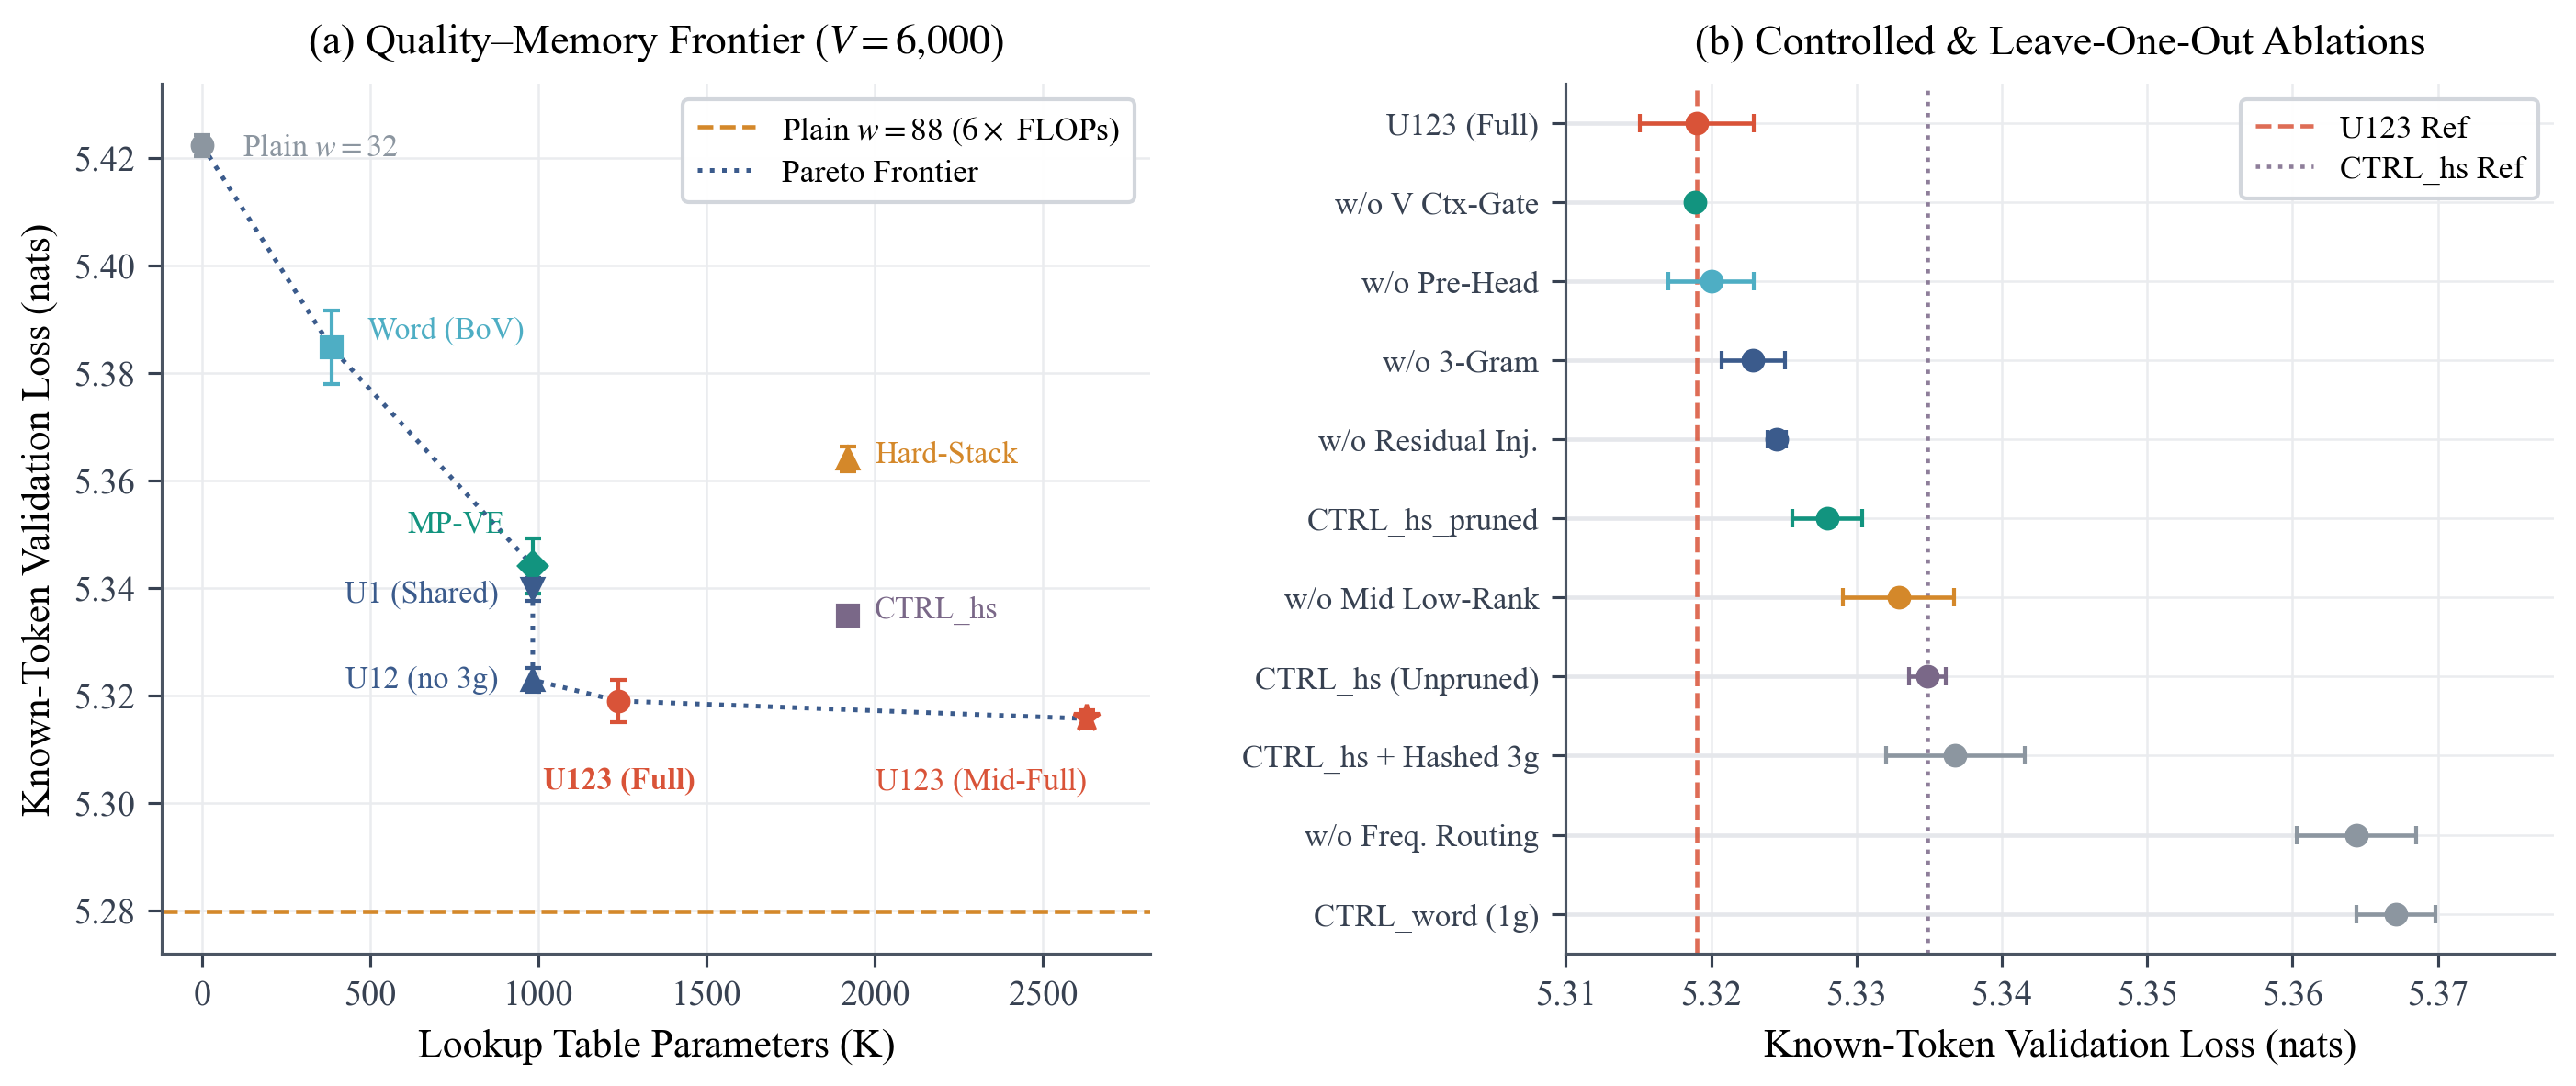
\includegraphics[width=0.49\linewidth]{../figs_v5/fig4_method.png}\hfill
    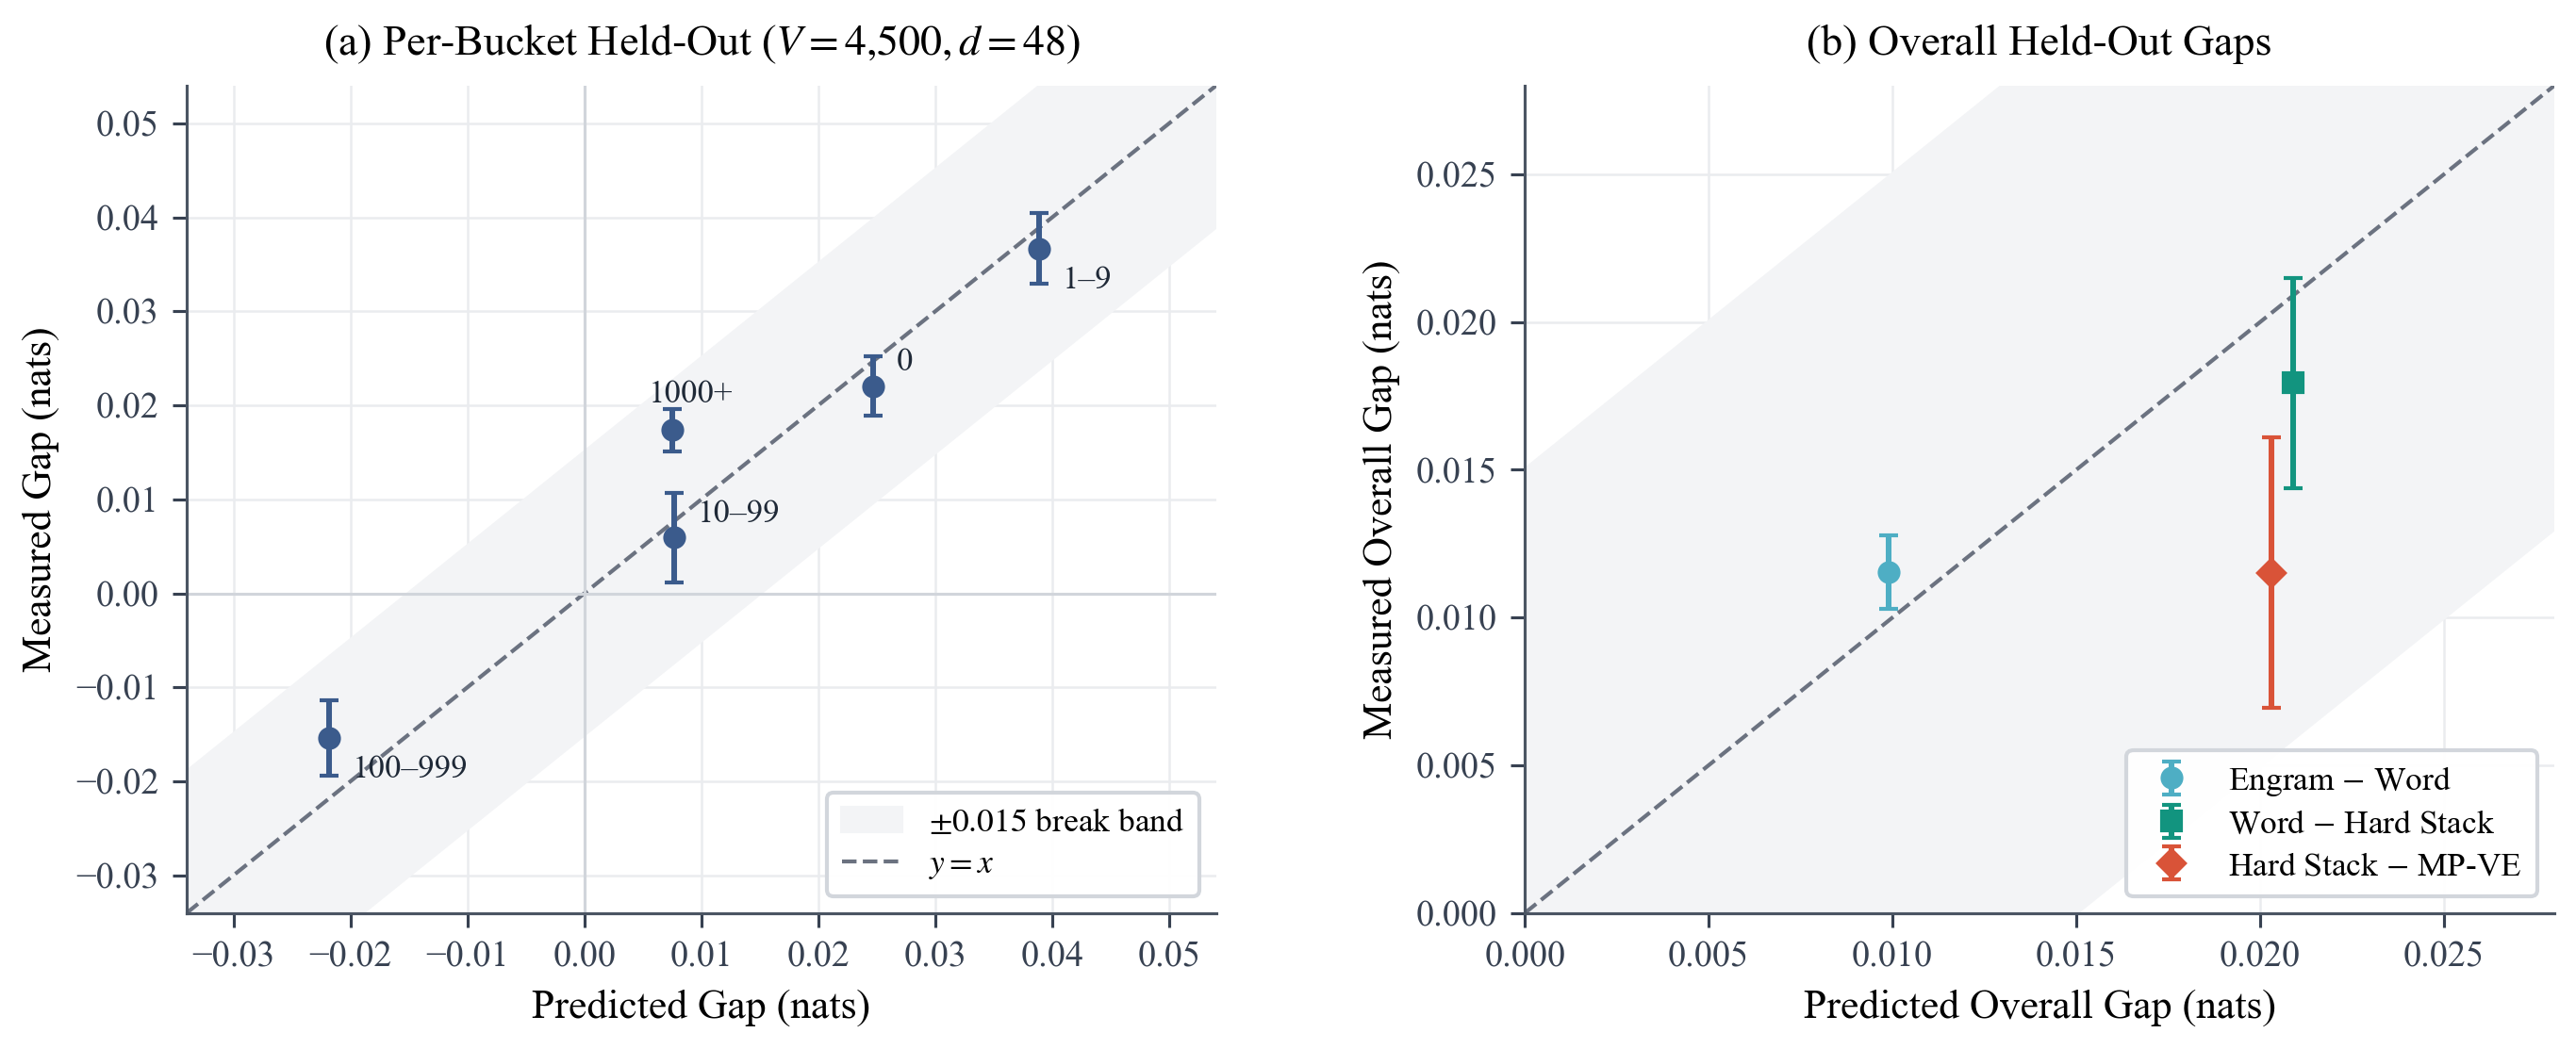
\includegraphics[width=0.49\linewidth]{../figs_v5/fig5_heldout.png}
    \caption{左（Fig.~4）：$L=4,w=32,V=6{,}000$ 上 \texttt{U1}、\texttt{U123} 与 \texttt{CTRL\_word/CTRL\_hs} 及 Equal-Weights 参考线对比；右（Fig.~5）：Round 30 预注册跨词表持出检验（$V=4{,}500, d=48, L=4$），全部预测符号与绝对误差均落在 $0.015$ nats 阈值之内。}
    \label{fig:fig45}
\end{figure}

% ============================================================
\section{全词表 \texorpdfstring{$V=50{,}257$}{V=50,257} Bridge 实测与工程代价账本}
% ============================================================

\subsection{真实 FineWeb 1 亿 Token 语料的 Zipf--Heaps 账本}
小词表（$V\le 6{,}000$）存在大量 \texttt{<UNK>}，因此我们在真实 GPT-2 词表（$V=50{,}257$）的 $100\text{M}$ FineWeb 训练分片上完成了精确统计（\texttt{pairstat\_v50257.json}）：
\begin{itemize}
    \item \textbf{极度集中与显存账本：} $100\text{M}$ token 观测到 $11{,}508{,}089$ 个独立词对；其中仅有 $109{,}774$ 个（占独立词对的 \textbf{0.954\%}）达到 $\ge 100$ 次，却覆盖了验证集 \textbf{55.76\%} 的 token 位置；另有 $881{,}672$ 个词对处于 $10\text{--}99$ 次中频带。若暴力建全量 768 维 2-gram 表需 $8.8\text{B}$ 参数，完全不可行；通过三档剪枝分配与前 10\% 前缀筛选，可将全词表双/三元组表压缩至 $69\text{--}77\text{M}$ 量级，实现工程可运行。
    \item \textbf{交叉与长程覆盖外推：} 验证集 $\ge 100$ 次词对占比跨过 $50\%$ 发生在 $50\text{M}\text{--}100\text{M}$ tokens（$47.73\% \to 55.76\%$）；基于 $100\text{M}$ 统计向下界外推（将未见词对视作零概率），到 $2.0\text{B}\text{--}5.0\text{B}$ tokens 时成熟词对覆盖率预计达 \textbf{82.69\%--87.17\%}（该估计已通过 $10\text{M}\to 100\text{M}$ 的十倍盲测校准：预测 $55.59\%$ vs 实测 $55.76\%$，误差 $<0.2\%$）。
\end{itemize}

\subsection{\texorpdfstring{$30\text{M}$}{30M}-Token 全词表 Bridge 与三项拆解结果（图~\ref{fig:fig7} 与表~\ref{tab:bridge50k}）}
为直接检验全词表且无 \texttt{<UNK>} 环境下算法是否成立，我们在 $L=6, d=256, V=50{,}257$ 模型上跑通了 FineWeb \texttt{30M} tokens Bridge 实验（Seed 0，仅使用前 10\% 前缀计数路由）及实测吞吐基准：

\begin{table}[htbp]
\centering
\caption{全词表 $V=50{,}257$（FineWeb \texttt{30M} tokens，10\% 前缀计数，Seed 0）性能与实时吞吐/延迟实测}
\label{tab:bridge50k}
\resizebox{\linewidth}{!}{%
\begin{tabular}{lccccccc}
\toprule
\textbf{对比臂} & \textbf{Val Loss} & \textbf{\texttt{pc\_0}} & \textbf{\texttt{pc\_100}} & \textbf{总参（表参）} & \textbf{B1 Seq256 (ms)} & \textbf{Train (tok/s)} & \textbf{归因与角色定位} \\
\midrule
\texttt{plain\_d256\_eqFLOP} & 4.9855 & 5.0715 & 4.7376 & 30.4M (0) & 15.68 & 40,610 & Equal Active FLOPs 主基线 \\
\texttt{word\_d256\_last2} & 4.8961 & 4.9432 & 4.6631 & 56.2M (25.7M) & 12.74 & 38,094 & 传统 1-gram 基线 \\
\texttt{mp\_ve\_d256\_prefix10} & 4.8697 & 4.9314 & 4.6254 & 99.8M (69.4M) & 14.00 & 34,035 & 三档 MP-VE（无共享/3g） \\
\texttt{U1\_shared\_d512\_all6} & 4.8658 & 4.9305 & 4.6271 & 101.4M (69.4M) & 15.29 & 31,203 & 跨层共享消融 \\
\texttt{plain\_d384\_eqWeights} ($2.25\times$ FLOPs) & 4.8570 & 4.9012 & 4.6261 & 49.2M (0) & 13.51 & 34,858 & 加宽密集主干对照 \\
\texttt{CTRL\_hs\_d256\_prefix10} & 4.8324 & 4.9028 & 4.6003 & 110.7M (76.9M) & 18.32 & 24,645 & 哈希+适配框架对照 \\
\texttt{CTRL\_hs\_pruned\_d256\_prefix10} & 4.8263 & 4.8597 & 4.6064 & 110.7M (76.9M) & 18.30 & — & 加入成熟度剪枝去污染 \\
\textbf{\texttt{U123\_d256\_prefix10}} & \textbf{4.8234} & \textbf{4.8537} & \textbf{4.5833} & 110.2M (76.5M) & 18.93 & 24,976 & \textbf{完整方法：剪枝 + 精确去碰撞} \\
\bottomrule
\end{tabular}%
}
\end{table}

\begin{figure}[htbp]
    \centering
    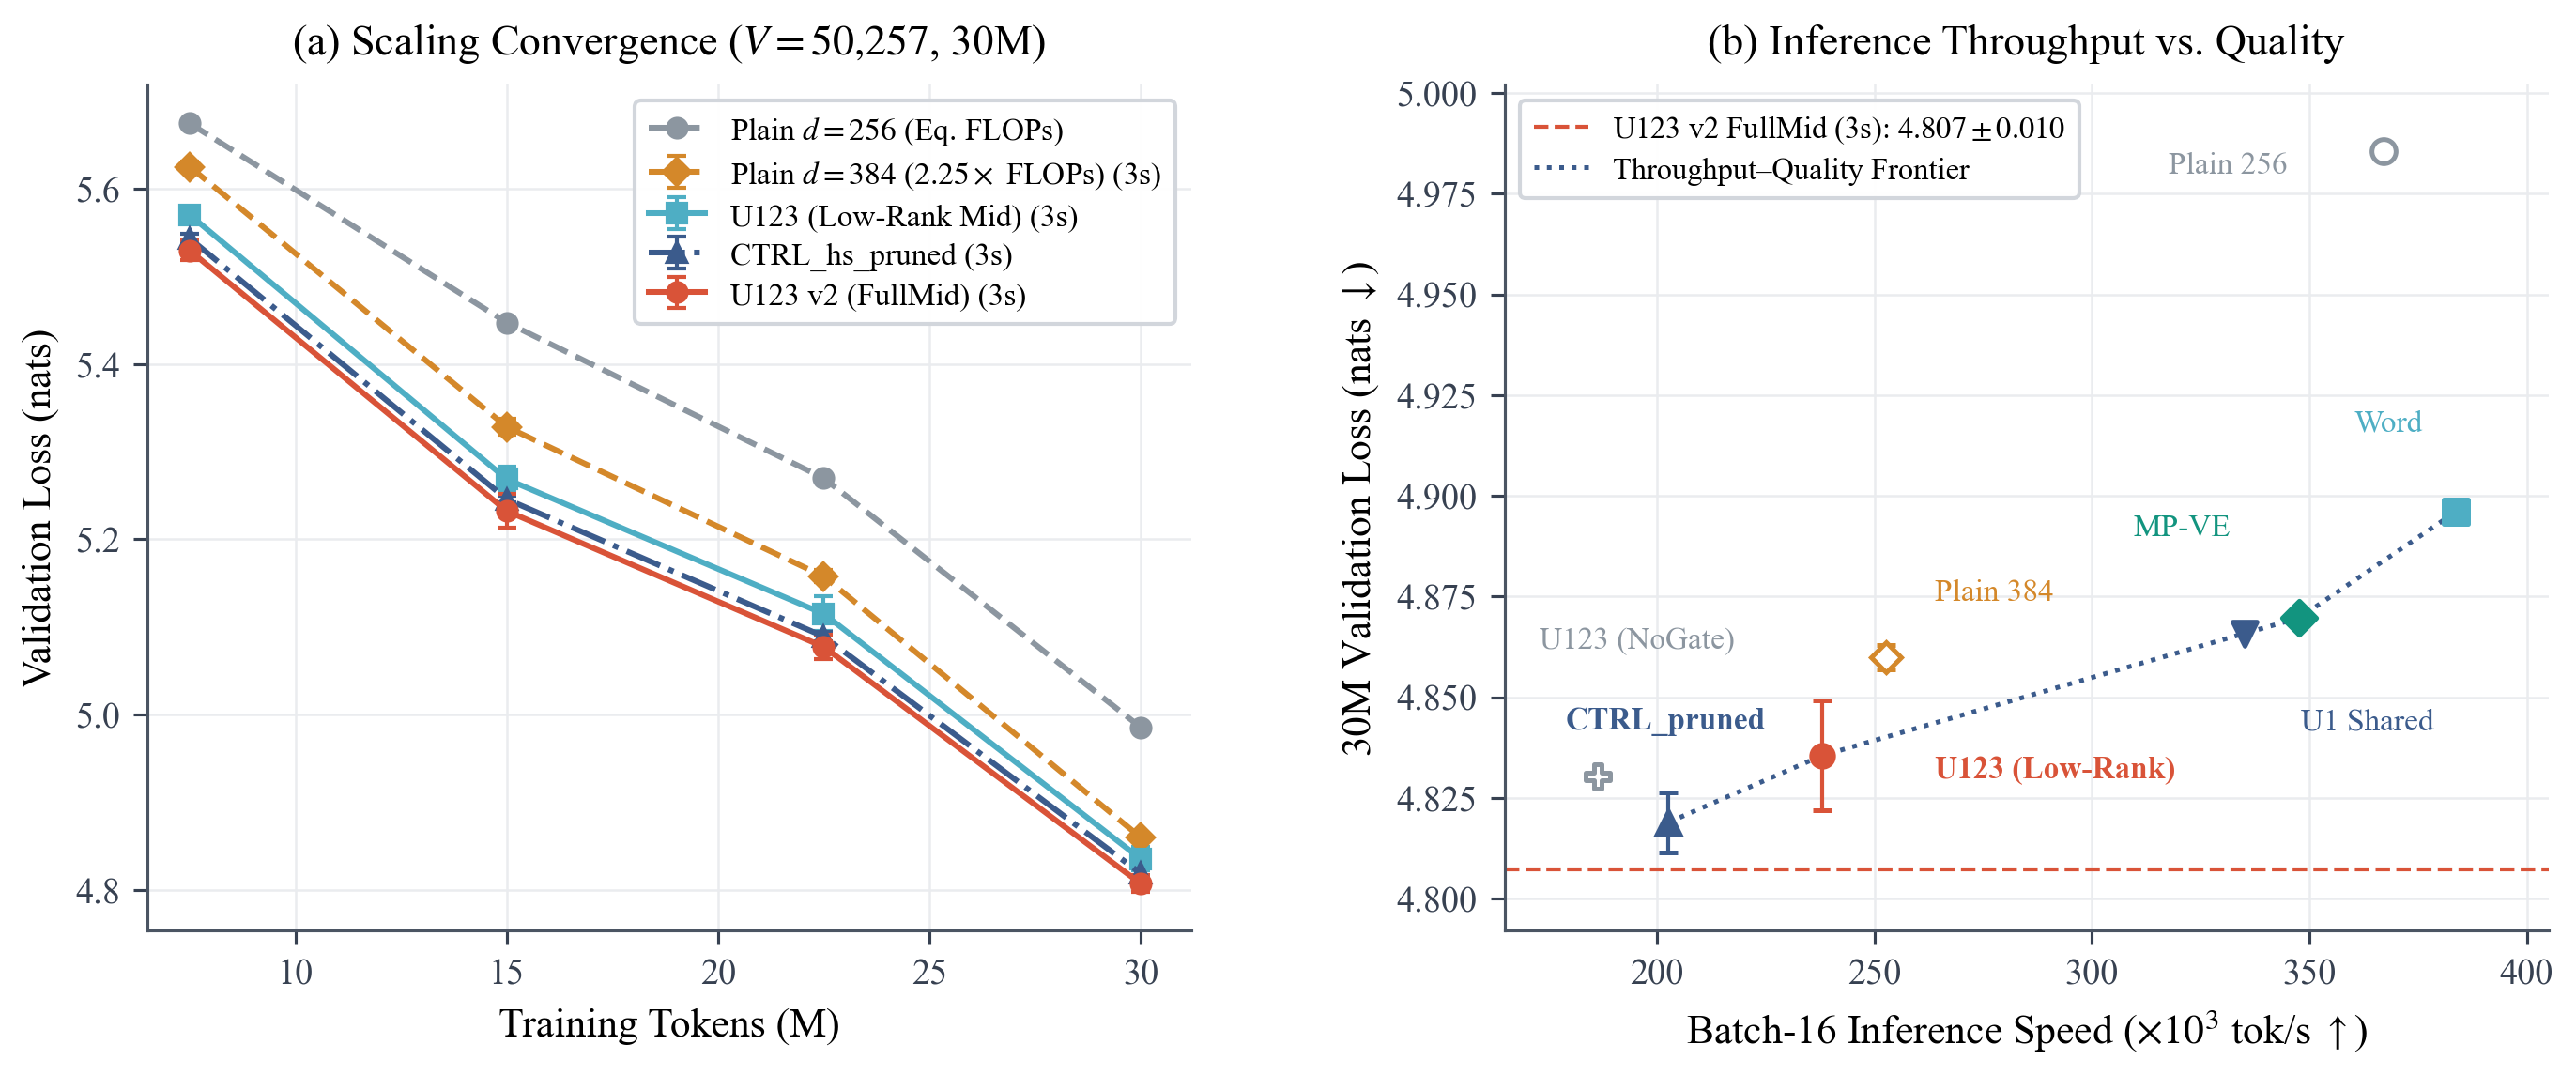
\includegraphics[width=0.88\linewidth]{../figs_v5/fig7_bridge.png}
    \caption{Fig.~7：全词表 $V=50{,}257$（$L=6, d=256$, 30M tokens）定向验证走势（Seed 0）。注意该图基线展示早期 \texttt{mp\_ve\_d256\_prefix10}（4.8697）；随后补充的 \texttt{U123}（4.8234）不仅比等激活计算量基线 \texttt{plain\_d256} 降低 $0.1621$ nats，亦超越 $2.25\times$ 激活算力的加宽基线 \texttt{plain\_d384}（4.8570）$+0.0336$ nats，并在 30M 处反超 \texttt{CTRL\_hs}。}
    \label{fig:fig7}
\end{figure}

表~\ref{tab:bridge50k} 的检查点轨迹直接印证了第 3.2 节提出的 $T_{\text{cross}}$ 分解：
\begin{itemize}
    \item \textbf{先输后赢的交叉轨迹：} 在 $7.5\text{M}$ tokens 处，\texttt{U123} 因宽表与低秩投影预热整体落后 \texttt{CTRL\_hs} $-0.0183$（$15\text{M}$ 追至 $-0.0001$，$22.5\text{M}$ 反超 $+0.0041$，$30\text{M}$ 扩大至 $+0.0090$）。
    \item \textbf{三项严格拆解：} \texttt{CTRL\_hs\_pruned} 较 \texttt{CTRL\_hs} 提升 $+0.0061$，几乎全部来自在未成熟位置 \texttt{pc\_0} 的剪枝去污染（\textbf{$+0.0431$} nats）；而 \texttt{U123} 相比 \texttt{CTRL\_hs\_pruned} 的净增 $+0.0029$ 内部包含清晰的结构分工——中频预热期在 \texttt{pc\_10} 暂时让出 $-0.0233$，但凭借精确 \texttt{2g/3g} 消除哈希碰撞，在成熟桶 \texttt{pc\_100} 上大胜 \textbf{$+0.0231$} nats，在 \texttt{pc\_1000} 上胜出 \textbf{$+0.0145$} nats。
    \item \textbf{诚实汇报工程开销（\texttt{latency\_v50257.json}）：} 推理阶段（\texttt{torch.no\_grad}, RTX 4070）只需执行 $\mathcal{O}(1)$ 嵌入读取，Batch-16 推理吞吐保持在 \textbf{224K--327K tok/s}（对比 \texttt{plain\_d256} 287K tok/s）；而\textbf{训练阶段}由于需要对 $69\text{--}77\text{M}$ \texttt{fp32} 表主权重执行 Dense Adam 更新与梯度 Scatter，导致 \texttt{U123/CTRL\_hs} 训练吞吐较 \texttt{plain\_d256} 下降约 $38\%$（$24.9\text{k}$ vs $40.6\text{k tok/s}$）。
\end{itemize}

% ============================================================
\section{下一阶段：\texorpdfstring{\texttt{125M × 2.5B}}{125M x 2.5B} 云端实验设计与协作分工}
% ============================================================

\subsection{云端 4-GPU 规模化验证矩阵与硬件预算}
前述所有结果均已在本地（最多至 $30\text{M}$ tokens）跑通验证；要在顶会（ICML / TMLR / COLM）上建立无懈可击的 Scaling 证据，下一核心里程碑是在 4 卡 A100/H100 节点上完成 \textbf{125M 参数主干 $\times$ 2.5B FineWeb tokens} 验证（代码已在根目录 \texttt{train\_125m.py} 验证因果零泄漏，支持 \texttt{--smoke} 全臂一键通过）：
\begin{enumerate}
    \item \textbf{数据与磁盘预算（\texttt{download\_data.py}）：} 多线程下载并校验 26 个 FineWeb 分片（约 50 GB 训练分片 + 模型日志 $\approx 60\text{ GB}$）。
    \item \textbf{分波次（Multi-Wave）实验队列（\texttt{run\_125m\_experiments.sh}）：}
    \begin{itemize}
        \item \textbf{Wave 1（主线四臂，Seed 0）：} \texttt{plain}（$d=768, 124.7\text{M}$ 等激活 FLOPs）、\texttt{u123}、\texttt{ctrl\_hs\_pruned}、\texttt{word}；
        \item \textbf{Wave 2（严格归因与算力界限）：} \texttt{ctrl\_hs}（未剪枝对照）、\texttt{ctrl\_word}（纯 1-gram 适配框）、\texttt{plain\_eq\_weights}（$d=1024$，约 $220\text{M}$ 等总参数主干）；
        \item \textbf{Wave 3（补充消融与多 Seed）：} \texttt{mp\_ve}、\texttt{u1} 以及对核心 4 臂补齐 Seed 1 / Seed 2 统计显著性。
    \end{itemize}
    \item \textbf{待补齐的理论与下游评测：}
    \begin{itemize}
        \item 运行 \texttt{experiments/run\_theory\_tests\_L\_M\_rho.py} 完成 $M \in \{6\text{k}, 24\text{k}, 96\text{k}\}$ 碰撞标度与 $L \in \{2, 4, 6\}$ 深度共享梯度相关性检验；
        \item 在 $2.5\text{B}$ 检查点补充下游任务基准（\texttt{lm-eval}: LAMBADA / HellaSwag / PIQA / ARC-Easy），验证 PPL 下降是否真实传导至语言推理准确度。
    \end{itemize}
\end{enumerate}

\subsection{预注册判定准则（Go / No-Go Criteria）}
\begin{itemize}
    \item \textbf{强正面成立条件：} 若在 \texttt{2.5B} 处（此时 $>82\%$ 位置已越过 100 次更新门槛）\texttt{u123} 跨多 seed 稳定击败 \texttt{ctrl\_hs\_pruned} 与 \texttt{ctrl\_word}，并复现“剪枝保 \texttt{pc\_0}、精确表赢 \texttt{pc\_100/1000}”的两段式分解，同时在接近等推理延迟下逼近或局部追平 $2.25\times$ 算力的 \texttt{plain\_eq\_weights}，则直接支撑顶会终稿冲刺；
    \item \textbf{局部证伪退化预案：} 若在长程 \texttt{2.5B} 下精确键表的相对增益衰减或深度缩放 $\rho_{\text{noise}}$ 过高，则按科学诚信准则将对应组件定格为“中等尺度现象学规律及失效边界”，同样形成扎实的技术报告与消融基准资产。
\end{itemize}

\subsection{给新合作者的代码仓库速览}
仓库结构及协作规范（详见 \texttt{README.md}、\texttt{CONTRIBUTING.md} 与 \texttt{CLOUD\_AGENT\_HANDOFF.md}）如下：
\begin{itemize}
    \item \textbf{根目录：} 云端 125M 主训练器（\texttt{train\_125m.py}）、并发数据下载器（\texttt{download\_data.py}）与 4-GPU 启动脚本（\texttt{run\_125m\_experiments.sh}）；
    \item \textbf{\texttt{experiments/} 与 \texttt{results/}：} 全部本地/Bridge 实验脚本与对应 JSON 产出（1-to-1 对应，禁止提交孤儿数据）；
    \item \textbf{\texttt{analysis/} 与 \texttt{figs\_v5/}：} 运行 \texttt{python analysis/make\_figs\_v5.py} 与 \texttt{python analysis/theory\_cstar\_analysis.py} 即可在无 GPU 环境下秒级复现全套出版级图表与理论分析。
\end{itemize}

\end{document}
